%% Beamer template
%% Author: Markus Solbach
%% eMail: solbach@eecs.yorku.ca

\documentclass{beamer}
\usetheme{Dresden}

\usepackage{appendixnumberbeamer}

\addtobeamertemplate{navigation symbols}{}{%
    \usebeamerfont{footline}%
    \usebeamercolor[fg]{footline}%
    \hspace{1em}%
    \insertframenumber/\inserttotalframenumber
}

\title{Template Title}
\author{John Doe}
\subject{Presentation Programs}

\institute[Some University]{Some University}

\begin{document}

\setbeamertemplate{headline}{}

\begin{frame}
  \maketitle
\end{frame}


\begin{frame}
	\tableofcontents
\end{frame}

\section{Introduction}
\begin{frame}
    \frametitle{Introduction}
\end{frame}

\begin{frame}
\frametitle{Introduction}
  Some text
      \begin{itemize}
        \item Point 1
        \begin{itemize}
          \item Sub-Point
          \item Sub-Point
          \item Sub-Point
          \item Sub-Point
          \item Sub-Point
        \end{itemize}
        \item Poiny 2
      \end{itemize}
\end{frame}

\begin{frame}
\frametitle{Introduction}
    Image Example - Full
    \begin{figure}[ht]
      \centering
        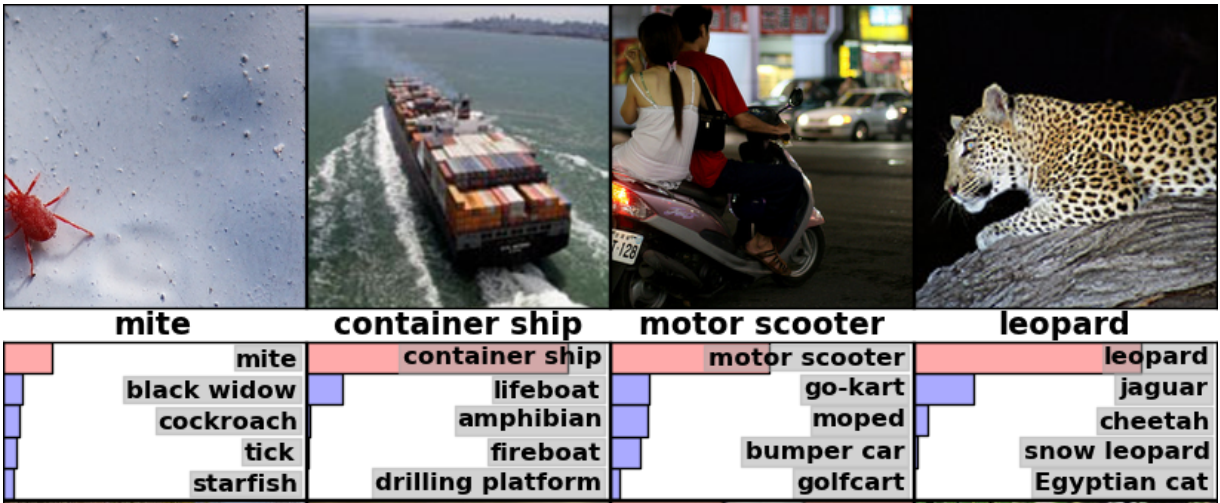
\includegraphics[width=0.9\textwidth]{img/alex.png}
      \caption{AlexNet results. \tiny{Source: \url{https://www.tensorflow.org} (17.09.16)} }
    \end{figure}
\end{frame}

\section{A new World}
\begin{frame}
\frametitle{A new World}
\end{frame}

\begin{frame}
\frametitle{A new World}
Custom bullet points
\begin{columns}
    \begin{column}{0.65\textwidth}
      \begin{itemize}
        \item [IN] Images
        \item [OUT] Data
      \end{itemize}
    \end{column}

    \begin{column}{0.35\textwidth}
      \begin{figure}[ht]
        \centering
        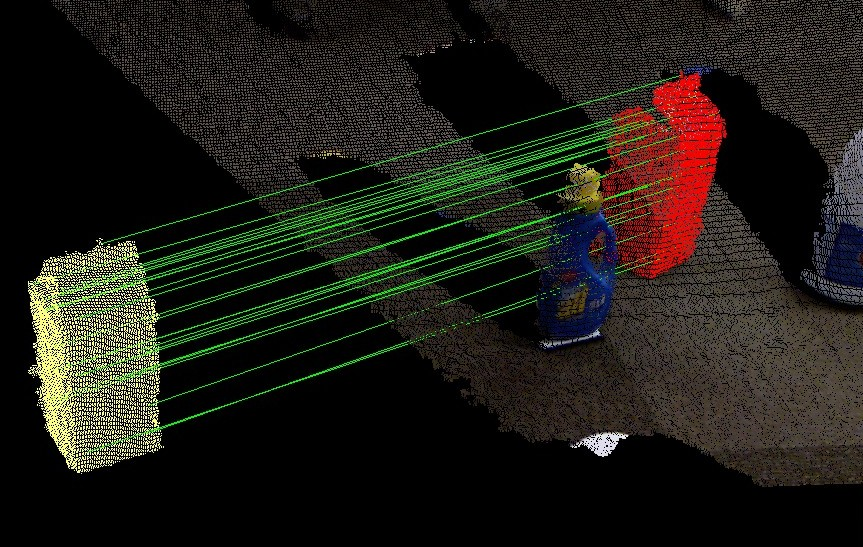
\includegraphics[width=0.8\textwidth]{img/pcl.jpg}
        \caption{3D recognition. \tiny{Source: \url{http://www.pcl.org/} (17.09.16)} }
      \end{figure}
    \end{column}
  \end{columns}
\end{frame}

\begin{frame}
    \frametitle{A new World}
    Math, math, math and \LaTeX
    \begin{equation}
      \sum_{k=1}^{n}{k} = \cfrac{n}{2}(n+1)
    \end{equation}
\end{frame}

\begin{frame}
    \frametitle{A new World}
    Math, math, math and \LaTeX and references
    \begin{equation}
      \sum_{k=1}^{n}{k} = \cfrac{n}{2}(n+1)
    \end{equation}

    \begin{itemize}
      \item Text (template)
      \begin{itemize}
        \item [\color{red}--] proper minus
        \item [\color{red}--] proper minus
        \begin{itemize}
          \item Time
          \item Citation \cite{martin1997island}
        \end{itemize}
      \end{itemize}
    \end{itemize}
\end{frame}

\section{Future}
\begin{frame}
\frametitle{Future}

\end{frame}

\begin{frame}
\frametitle{Future}
  \begin{itemize}
    \item Item 1 (\color{blue} Done\color{black})
    \begin{itemize}
      \item 20 Classes
      \item Inline Math: $> 9000$ Images $\approx$ 450 Images per Class
    \end{itemize}
    \item Item 2 (\color{orange} In progress\color{black})
    \begin{itemize}
      \item Example Implementation
      \item Debug $\hookrightarrow$ Code
    \end{itemize}
    \item Item 3 (\color{blue} Done\color{black})
    \begin{itemize}
      \item Text (test)
    \end{itemize}
    \item [To Do] Item 4
  \end{itemize}
\end{frame}

%Bibliography
\begin{frame}
  \frametitle{References}

  % Short
  %\bibliographystyle{alpha}

  % Full
  \bibliographystyle{apalike}
  \bibliography{templ}
\end{frame}

%% everything beyond \appendix is not shown in the table of content and is not counted
\appendix

\begin{frame}
\frametitle{Appendix}
  Some additional material!
\end{frame}


\end{document}
